\section{System Evaluation And Case Study}
\label{sec:evo} 
\par  In the case study, we use two concrete tasks to demonstrate how investors can apply FKAP to the analysis of movie box office.
\textbf{Task 1: Movie Inclusion.} It's important for investors to analyze the performance of a movie. Movie performance not only refers to box office income, word of mouth, but also includes the changes in the audience and the change of the influence of the director during the screening process.

\begin{figure}[!htbp]
\centering
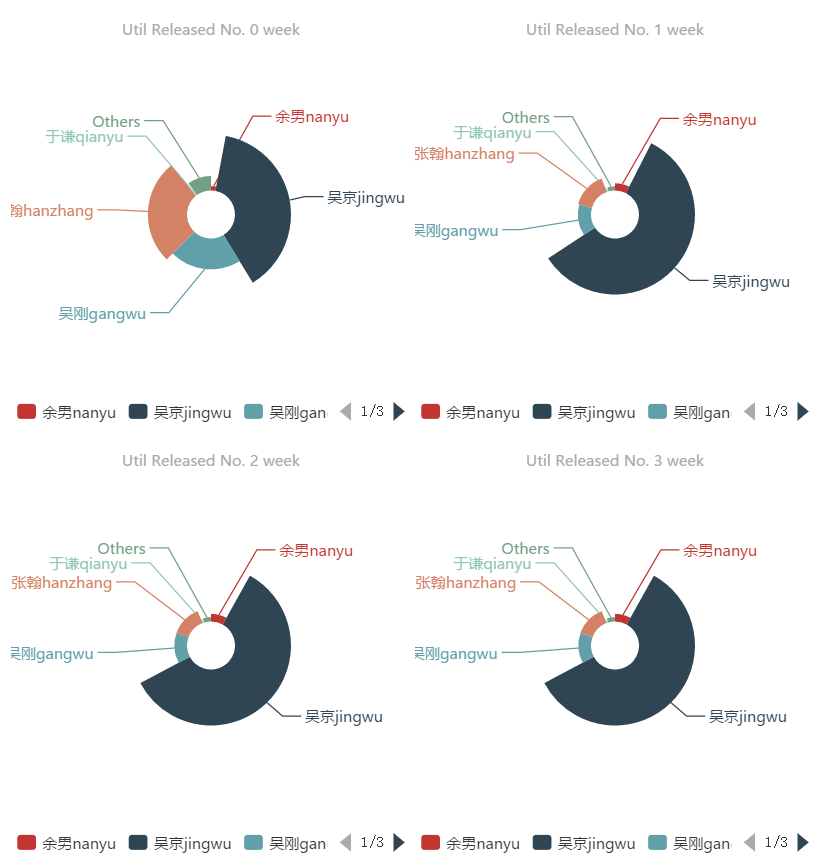
\includegraphics[width=0.8\columnwidth]{case1.png}
\caption{Dynamic Impact of Wolf Warriors II}
\label{fig:case1}
\end{figure}

\par Fig.4 shows dynamic impact of creators in "Wolf Warriors II". Before the movie released (week 0), the attentions people payed to Hans Zhang, Gang Wu and Jason Wu were equal while with the movie's release and the increase in the heat of the film, more and more people went to the movies for the sake of Jason Wu. Meanwhile, the dynamic influence process can reflect a major change in the importance of the movie. We can see that Jason Wu has greatly improved his value through the movie himself. To some extent, Jason Jing has more box office attractiveness, and investing in the actor's next movie is very likely to get high box office gains.

\textbf{Task 2: Evaluation of investment quality.} Investors usually need to assess the movie's expected box office and measure the actor's return on investment. Because there is a strong correlation between movie box office and audience feedback, the box office of the first week is less affected by audience feedback, so the first week box office can be regarded as the baseline of box office. The first week box office prediction can measure the expected revenue of the movie, and the actor replacement module can help investors to screen the appropriate actors at the right price at the appropriate box office in the first week.